\documentclass{article}
\usepackage{tikz}
\usetikzlibrary{calc,shapes.multipart,chains,arrows}

\begin{document}

% Explication principe tableau cumulatif grâce à la géométrie

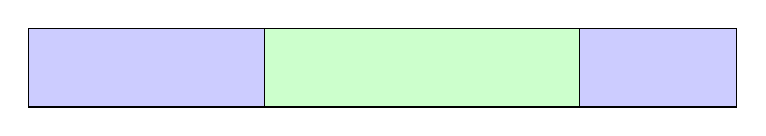
\begin{tikzpicture}
\fill[blue!20, draw=black] (-2,0) rectangle (7,1);
\fill[green!20, draw=black] (1,0) rectangle (5,1);
\end{tikzpicture}

\vspace{2cm}


\begin{tikzpicture}
\fill[white] (-2,0) rectangle (7,1);
\fill[green!20, draw=black] (1,0) rectangle (5,1);
\node at (3,-0.5) {$=$};
\end{tikzpicture}

\vspace{0.25cm}

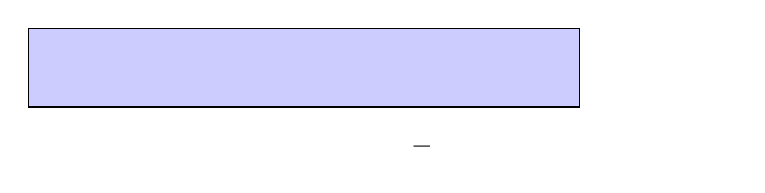
\begin{tikzpicture}
\fill[white] (-2,0) rectangle (7,1);
\fill[blue!20, draw=black] (-2,0) rectangle (5,1);
\node at (3,-0.5) {$-$};
\end{tikzpicture}

\vspace{0.25cm}


\begin{tikzpicture}
\fill[white] (-2,0) rectangle (7,1);
\fill[blue!20, draw=black] (-2,0) rectangle (1,1);
\end{tikzpicture}

% Représentation des intervalles nécessaires

\newpage

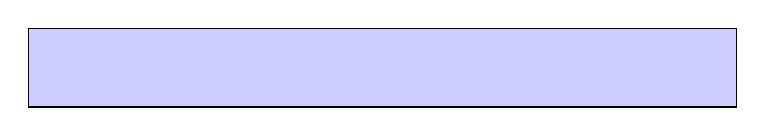
\begin{tikzpicture}
\fill[blue!20, draw=black] (-2,0) rectangle (7,1);
\end{tikzpicture}

\vspace{1cm}
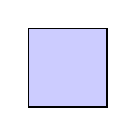
\begin{tikzpicture}
\fill[blue!20, draw=black] (-2,0) rectangle (-1,1);
\end{tikzpicture}

\vspace{0.25cm}
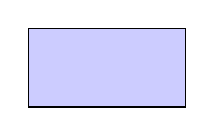
\begin{tikzpicture}
\fill[blue!20, draw=black] (-2,0) rectangle (0,1);
\end{tikzpicture}

\vspace{0.25cm}
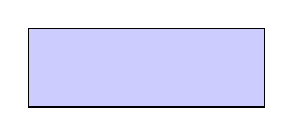
\begin{tikzpicture}
\fill[blue!20, draw=black] (-2,0) rectangle (1,1);
\end{tikzpicture}

\vspace{0.25cm}
\begin{tikzpicture}
\node (2, 1) {$...$};
\end{tikzpicture}

\vspace{0.25cm}
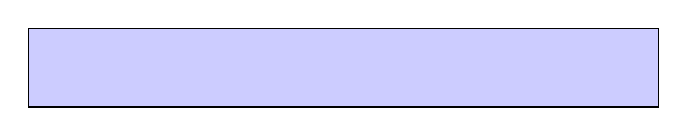
\begin{tikzpicture}
\fill[blue!20, draw=black] (-2,0) rectangle (6,1);
\end{tikzpicture}

\vspace{0.25cm}
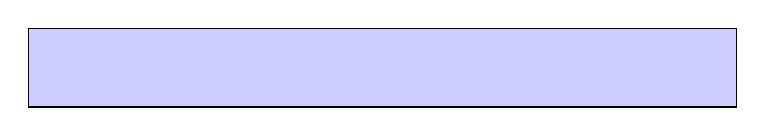
\begin{tikzpicture}
\fill[blue!20, draw=black] (-2,0) rectangle (7,1);
\end{tikzpicture}


\end{document}